\begin{frame}
\frametitle{Data and representation}
\begin{columns}
    \begin{column}{0.4\textwidth}
        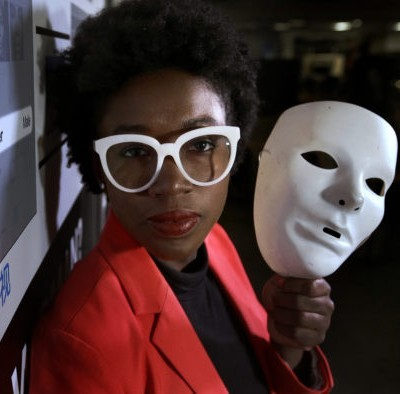
\includegraphics[width=1\textwidth]{./misc_images/joy_buolamwini.jpg}
    \end{column}
    \begin{column}{0.59\textwidth}
        When Joy Buolamwini was a computer science undergrad at Georgia Tech in the early 2010s, she worked on an assignment to recognise emotions in faces. The problem was that the face recognition library she used would not detect her own face, until she held up a white mask in front of her face.
        \\~\\
        At the time, many libraries were trained on the \emph{Labelled Faces in the Wild} database. It turned out that there are twice as many images of George W. Bush in the dataset as there are all of Black women combined.
    \end{column}
\end{columns}
\end{frame}